% !TEX root = main.tex
\section{Link Budget}
\label{sec:link_budget}
The link budget for the system is shown in table \ref{tab:link_budget}. The system is designed to operate indoors with a distance of 5 meters between transmitter and receiver. Table \ref{tab:link_budget} shows losses from propagation, loss in TX and RX, and some estimated key parameters at the receiver. 

In this demonstration, the transmit power is varied in order to simulate changes in the radio channel while the physical radio link is fixed. Hence no fading statistics is included in the link budget. The stated values are based on the transmit power used for high data rate transmission corresponding to the best simulated state of the radio channel. 

% !TEX root = main.tex
% Table generated by Excel2LaTeX from sheet 'Link Budget'
\begin{table*}[htbp]
  \centering
  \caption{Link Budget}
    \begin{tabular}{lccccr}
    \rowcolor[rgb]{ 0,  0,  0} \textcolor[rgb]{ 1,  1,  1}{\textbf{TX Loss}} & \textcolor[rgb]{ 1,  1,  1}{\textbf{Variable}} & \textcolor[rgb]{ 1,  1,  1}{\textbf{Units}} & \multicolumn{1}{p{13.915em}}{\textcolor[rgb]{ 1,  1,  1}{\textbf{Equation}}} & \multicolumn{2}{c}{\textcolor[rgb]{ 1,  1,  1}{\textbf{Value}}} \\
    \rowcolor[rgb]{ 0,  0,  0} \textcolor[rgb]{ 1,  1,  1}{} & \textcolor[rgb]{ 1,  1,  1}{} & \textcolor[rgb]{ 1,  1,  1}{} & \textcolor[rgb]{ 1,  1,  1}{} & \multicolumn{1}{p{3.75em}}{\textcolor[rgb]{ 1,  1,  1}{\textbf{QPSK}}} & \multicolumn{1}{p{4.5em}}{\textcolor[rgb]{ 1,  1,  1}{\textbf{QAM64}}} \\
    PA Power & $P_{PA}$ & dBm   &       & \multicolumn{2}{c}{10} \\
    TX Connector Loss & $L_{ConT}$ & dB    & \multicolumn{1}{p{13.915em}}{from connector data sheet} & \multicolumn{2}{c}{-0.3} \\
    TX Power & $P_T$ & dBm   & \multicolumn{1}{p{13.915em}}{$P_T=P_{PA}\cdot 2L_{ConT}$} & \multicolumn{2}{c}{9.4} \\
    TX Antenna Gain & $G_T$ & dBi   & \multicolumn{1}{p{13.915em}}{from antenna data sheet} & \multicolumn{2}{c}{3} \\
    Effective (Isotropic) Radiated Power & EIRP  & dBm   & \multicolumn{1}{p{13.915em}}{$\text{EIRP} = P_TG_T$} & \multicolumn{2}{c}{12.4} \\
    \rowcolor[rgb]{ 0,  0,  0} \multicolumn{3}{l}{\textcolor[rgb]{ 1,  1,  1}{\textbf{Path Loss, ITU Indoor Propagation Loss Model}}} & \textcolor[rgb]{ 1,  1,  1}{} & \textcolor[rgb]{ 1,  1,  1}{} & \textcolor[rgb]{ 1,  1,  1}{} \\
    Distance & $d$   & m     &       & \multicolumn{2}{c}{10} \\
    Floor loss factor & $Pf(n)$ & dB    &       & \multicolumn{2}{c}{0} \\
    Distance power loss coefficient & $N$   &       &       & \multicolumn{2}{c}{38} \\
    Total ITU path loss & $L_P$ & dB    &       & \multicolumn{2}{c}{-77.66} \\
    \rowcolor[rgb]{ 0,  0,  0} \textcolor[rgb]{ 1,  1,  1}{\textbf{RX Loss}} & \textcolor[rgb]{ 1,  1,  1}{} & \textcolor[rgb]{ 1,  1,  1}{} & \textcolor[rgb]{ 1,  1,  1}{} & \textcolor[rgb]{ 1,  1,  1}{} & \textcolor[rgb]{ 1,  1,  1}{} \\
    RX antenna gain & $G_R$ & dBi   &       & \multicolumn{2}{c}{3} \\
    RX connector loss & $L_{ConR}$ & dB    &       & \multicolumn{2}{c}{-0.3} \\
    Total RX Loss & $L_R$ & dB    &       & \multicolumn{2}{c}{2.4} \\
          &       &       &       & \multicolumn{2}{c}{} \\
    Total Received Power & $P_R$ & dBm   & \multicolumn{1}{p{13.915em}}{$P_R = \text{EIRP}\cdot L_P \cdot L_R$} & \multicolumn{2}{c}{-62.86} \\
    \rowcolor[rgb]{ 0,  0,  0} \textcolor[rgb]{ 1,  1,  1}{\textbf{RX Noise}} & \textcolor[rgb]{ 1,  1,  1}{} & \textcolor[rgb]{ 1,  1,  1}{} & \textcolor[rgb]{ 1,  1,  1}{} & \textcolor[rgb]{ 1,  1,  1}{} & \textcolor[rgb]{ 1,  1,  1}{} \\
    Antenna Noise Density & $N_0$ & dbm/Hz & \multicolumn{1}{p{13.915em}}{Measured with spectrum analyser. Average of several single runs} & \multicolumn{2}{c}{-145.73} \\
    Antenna Total Noise Power & $N$   & dBm   & \multicolumn{1}{p{13.915em}}{$\text{N0}\cdot \text{BW}$} & \multicolumn{2}{c}{-97.806} \\
    RX Noise Figure & $NF$  & dB    & \multicolumn{1}{p{13.915em}}{From NI USRP-2901 datasheet} & \multicolumn{2}{c}{7.000} \\
    Small Scale fading margin & $M_{ssf}$ & dB    & \multicolumn{1}{p{13.915em}}{From measurements of RX power variations} & \multicolumn{2}{c}{9.400} \\
    \rowcolor[rgb]{ 0,  0,  0} \textcolor[rgb]{ 1,  1,  1}{\textbf{RX Properties}} & \textcolor[rgb]{ 1,  1,  1}{} & \textcolor[rgb]{ 1,  1,  1}{} & \textcolor[rgb]{ 1,  1,  1}{} & \textcolor[rgb]{ 1,  1,  1}{} & \textcolor[rgb]{ 1,  1,  1}{} \\
    Carrier-to-noise ratio & $C/N$ & dB    & \multicolumn{1}{p{13.915em}}{$C/N_0 = \frac{P_R}{N NF M_{ssf}}$} & \multicolumn{2}{c}{18.548} \\
    Eb over N0 & $E_b/N_0$ & dB    & \multicolumn{1}{p{13.915em}}{$\frac{E_b}{N_0} = \frac{C}{N} \frac{\Delta f}{R_b}$} & \multicolumn{1}{r}{13.666} & 8.893 \\
    Eb over N0 & $E_b/N_0$ & lin   &       & \multicolumn{1}{r}{23.262} & 7.749 \\
    Bit error rate & BER   &       &       & 8.56E-08 & 3.17E-04 \\
    \end{tabular}%
  \label{tab:link_budget}%

\end{table*}%


The value for connector loss is taken from the data sheet of a standard coaxial RF connector \cite{rfconnector}. The antenna gain value is taken from the data sheet \cite{antenna}.The transmit power, $P_{PA}$, was adjusted after measurements to obtain appropriate $\nicefrac{E_b}{N_0}$ at the receiver.

The estimated path loss constitutes solely of the propagation loss obtained from the ITU Indoor Propagations Loss Model \cite{itu_model}. The loss model consists of two adjustable factors, the distance power loss coefficient, $N$, and the floor loss penetration factor, $P_f(n)$. The latter is set to 0, and the former was set to 38 after calibrating the test environment. Figure \ref{fig:path_loss} shows the measured path loss and the prediction from the ITU model before and after adjusting the power loss coefficient.

\begin{figure}[htbp]
\begin{center}
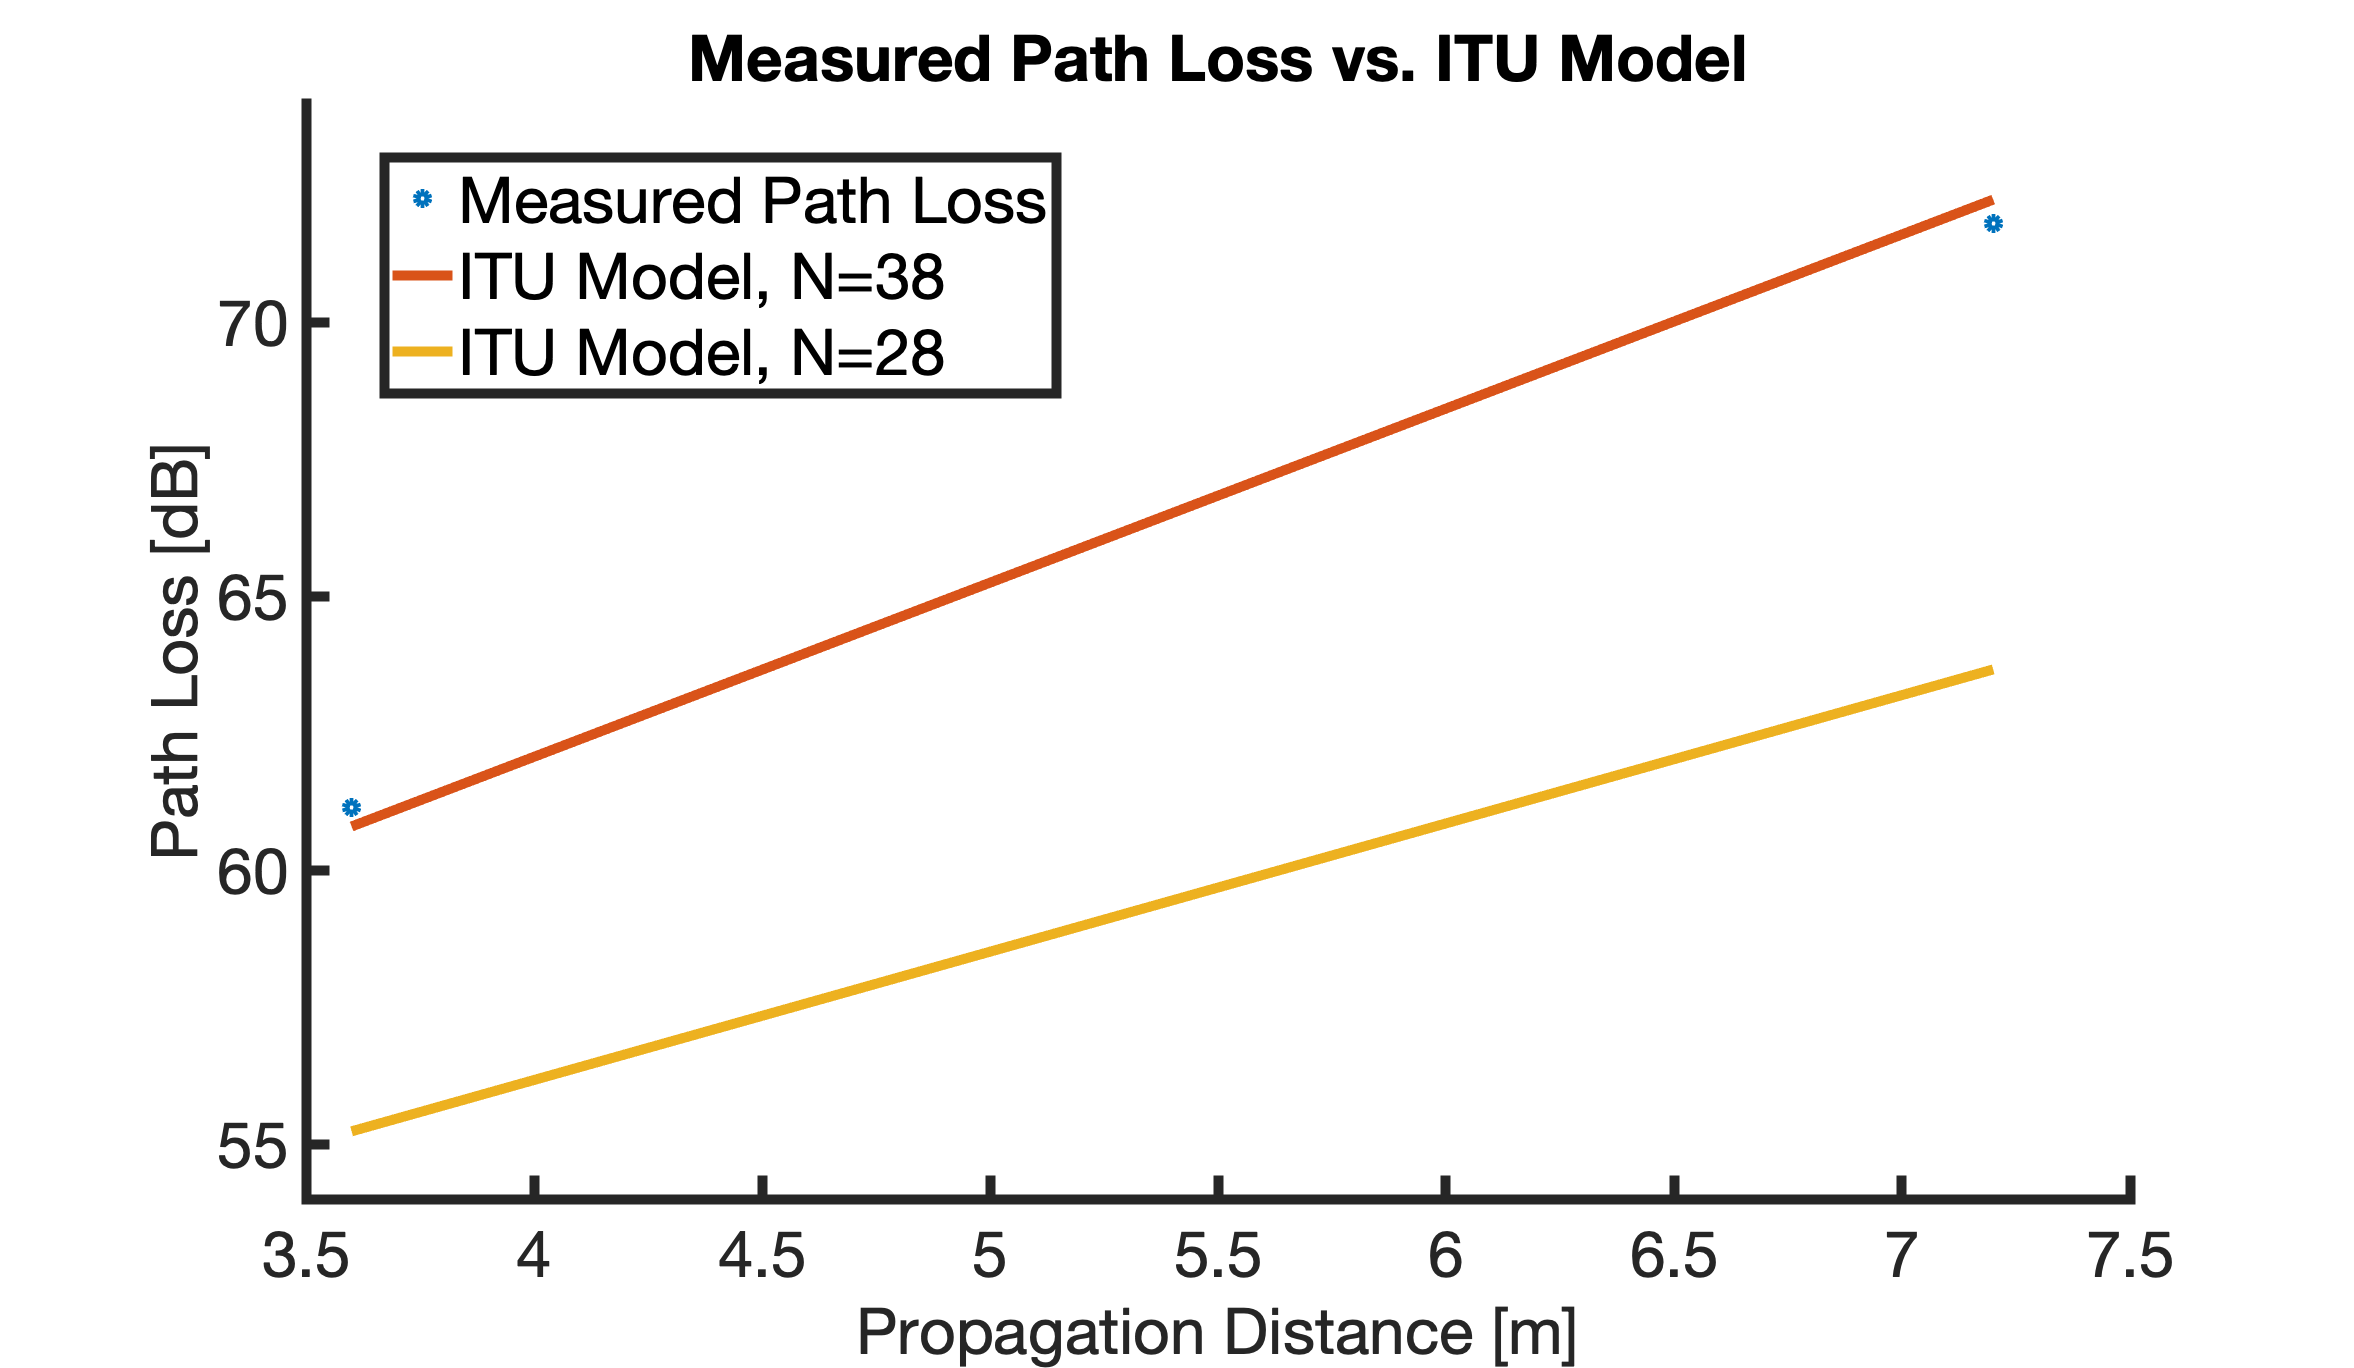
\includegraphics[width=0.85\linewidth]{PathLoss.png}
\caption{Measured path loss vs. estimated path loss from the ITU Indoor Propagations Loss Model, before and after adjusting the power loss coefficient}
\label{fig:path_loss}
\end{center}
\end{figure}

Other loss factors such as pointing loss and polarisation loss was considered, but measurements showed that the amount of reflections in the room made pointing and polarisation irrelevant to the received power. 
 
The antenna noise density was measured with a spectrum analyser and the estimated value was taken as an average of several single runs. The noise figure of the receiver is included to account for noise added by the radio hardware, with value taken from the data sheet. 
